\documentclass[tikz,border=0pt]{standalone}
% Shared visual language for the QCSD P3 methodology figures.
\usepackage{tikz}
\usepackage{lmodern}
\usetikzlibrary{arrows.meta,calc,decorations.pathreplacing,positioning,shapes.geometric}

\ifdefined\pdfoutput
  \ifnum\pdfoutput>0
    \ifdefined\pdfinfoomitdate
      \pdfinfoomitdate=1
    \fi
    \ifdefined\pdftrailerid
      \pdftrailerid{}
    \fi
    \ifdefined\pdfsuppressptexinfo
      \pdfsuppressptexinfo=15
    \fi
  \fi
\fi

\definecolor{qink}{HTML}{20242A}
\definecolor{qmid}{HTML}{666A70}
\definecolor{qlight}{HTML}{D7D8DA}
\definecolor{qpale}{HTML}{F2F2F1}
\definecolor{qamber}{HTML}{B8741A}
\definecolor{qamberpale}{HTML}{FFF1D7}
\definecolor{qteal}{HTML}{267985}
\definecolor{qtealpale}{HTML}{E5F2F3}
\definecolor{qred}{HTML}{B44A48}
\definecolor{qredpale}{HTML}{F8E7E6}

\tikzset{
  every node/.style={font=\fontsize{8.6}{10.2}\selectfont,text=qink,align=center},
  flow/.style={draw=qink,line width=.7pt,-{Latex[length=1.8mm,width=1.25mm]}},
  plain flow/.style={draw=qink,line width=.7pt},
  diagnostic/.style={draw=qteal,line width=.85pt,dashed,-{Latex[length=1.8mm,width=1.25mm]}},
  authoritative/.style={draw=qamber,line width=1.05pt,-{Latex[length=1.8mm,width=1.25mm]}},
  failure/.style={draw=qred,line width=.85pt,-{Latex[length=1.8mm,width=1.25mm]}},
  quiet outline/.style={draw=qlight,line width=.55pt,rounded corners=4pt},
  milestone/.style={circle,draw=qink,fill=white,line width=.7pt,inner sep=1.6pt},
  caption/.style={font=\fontsize{8.6}{10.2}\selectfont,text=qink},
  small note/.style={font=\fontsize{7.2}{8.5}\selectfont,text=qmid},
  tiny note/.style={font=\fontsize{6.6}{7.8}\selectfont,text=qmid},
}

% dvisvgm preserves these raw specials when the source is compiled to DVI.
% The PDF build intentionally omits them; its caption supplies the description.
\newcommand{\QCSDSvgMetadata}[2]{%
  \ifdefined\pdfoutput
    \ifnum\pdfoutput=0
      \special{dvisvgm:raw <title>#1</title>}%
      \special{dvisvgm:raw <desc>#2</desc>}%
    \fi
  \else
    \special{dvisvgm:raw <title>#1</title>}%
    \special{dvisvgm:raw <desc>#2</desc>}%
  \fi
}

% Neutral, project-owned pictograms.  They deliberately avoid product marks.
\tikzset{
  pics/client/.style={code={
    \fill[qink] (0,.25) circle (.16);
    \path[fill=qink,rounded corners=2.2pt]
      (-.30,-.30) -- (-.26,.00) arc[start angle=180,end angle=0,radius=.26]
      -- (.30,-.30) -- cycle;
  }},
  pics/tunnel/.style={code={
    \draw[qink,line width=1.1pt,rounded corners=2pt]
      (-.32,-.28) -- (-.32,.04) arc[start angle=180,end angle=0,radius=.32] -- (.32,-.28);
    \draw[qmid,line width=.6pt] (-.20,-.28) -- (-.20,.02)
      arc[start angle=180,end angle=0,radius=.20] -- (.20,-.28);
    \draw[qink,line width=.7pt] (-.36,-.28) -- (.36,-.28);
  }},
  pics/observer/.style={code={
    \draw[qink,line width=.85pt]
      (-.38,0) .. controls (-.17,.25) and (.17,.25) .. (.38,0)
      .. controls (.17,-.25) and (-.17,-.25) .. cycle;
    \fill[qink] (0,0) circle (.09);
  }},
  pics/gateway/.style={code={
    \path[draw=qink,fill=qpale,line width=.75pt,rounded corners=1.5pt]
      (-.34,-.25) rectangle (.34,.25);
    \draw[qink,line width=.65pt] (-.20,.03) -- (.20,.03);
    \fill[qink] (-.20,-.12) circle (.025);
    \fill[qink] (-.08,-.12) circle (.025);
    \fill[qink] (.04,-.12) circle (.025);
    \draw[qink,line width=.65pt] (.22,.25) -- (.22,.40);
  }},
  pics/server/.style={code={
    \path[draw=qink,fill=qpale,line width=.75pt]
      (-.27,-.36) rectangle (.27,.36);
    \draw[qmid,line width=.5pt] (-.18,.20) -- (.18,.20)
      (-.18,.02) -- (.18,.02) (-.18,-.16) -- (.18,-.16);
    \fill[qink] (.15,.27) circle (.022);
    \fill[qink] (.15,.09) circle (.022);
    \fill[qink] (.15,-.09) circle (.022);
  }},
  pics/globe/.style={code={
    \draw[qink,line width=.7pt] (0,0) circle (.31);
    \draw[qmid,line width=.45pt] (-.31,0) -- (.31,0);
    \draw[qmid,line width=.45pt] (0,-.31) .. controls (-.16,-.14) and (-.16,.14) .. (0,.31);
    \draw[qmid,line width=.45pt] (0,-.31) .. controls (.16,-.14) and (.16,.14) .. (0,.31);
  }},
  pics/capture/.style={code={
    \path[draw=qink,fill=white,line width=.65pt]
      (-.27,-.34) -- (-.27,.34) -- (.10,.34) -- (.27,.17) -- (.27,-.34) -- cycle;
    \draw[qmid,line width=.5pt] (.10,.34) -- (.10,.17) -- (.27,.17);
    \draw[qmid,line width=.55pt] (-.16,.08) -- (.15,.08)
      (-.16,-.04) -- (.08,-.04) (-.16,-.16) -- (.15,-.16);
  }},
  pics/dataset/.style={code={
    \path[draw=qink,fill=white,line width=.65pt] (-.31,-.25) rectangle (.25,.28);
    \path[draw=qmid,fill=white,line width=.5pt] (-.22,-.34) rectangle (.34,.19);
    \draw[qmid,line width=.5pt] (-.13,.10) -- (.13,.10)
      (-.13,-.02) -- (.20,-.02) (-.13,-.14) -- (.12,-.14);
  }},
  pics/classifier/.style={code={
    \foreach \y in {-.23,0,.23} { \fill[qink] (-.28,\y) circle (.045); }
    \foreach \y in {-.14,.14} { \fill[qink] (0,\y) circle (.045); }
    \foreach \y in {-.23,0,.23} { \fill[qink] (.28,\y) circle (.045); }
    \foreach \a in {-.23,0,.23} { \foreach \b in {-.14,.14}
      { \draw[qmid,line width=.35pt] (-.235,\a) -- (-.045,\b); } }
    \foreach \a in {-.14,.14} { \foreach \b in {-.23,0,.23}
      { \draw[qmid,line width=.35pt] (.045,\a) -- (.235,\b); } }
  }},
}


\begin{document}
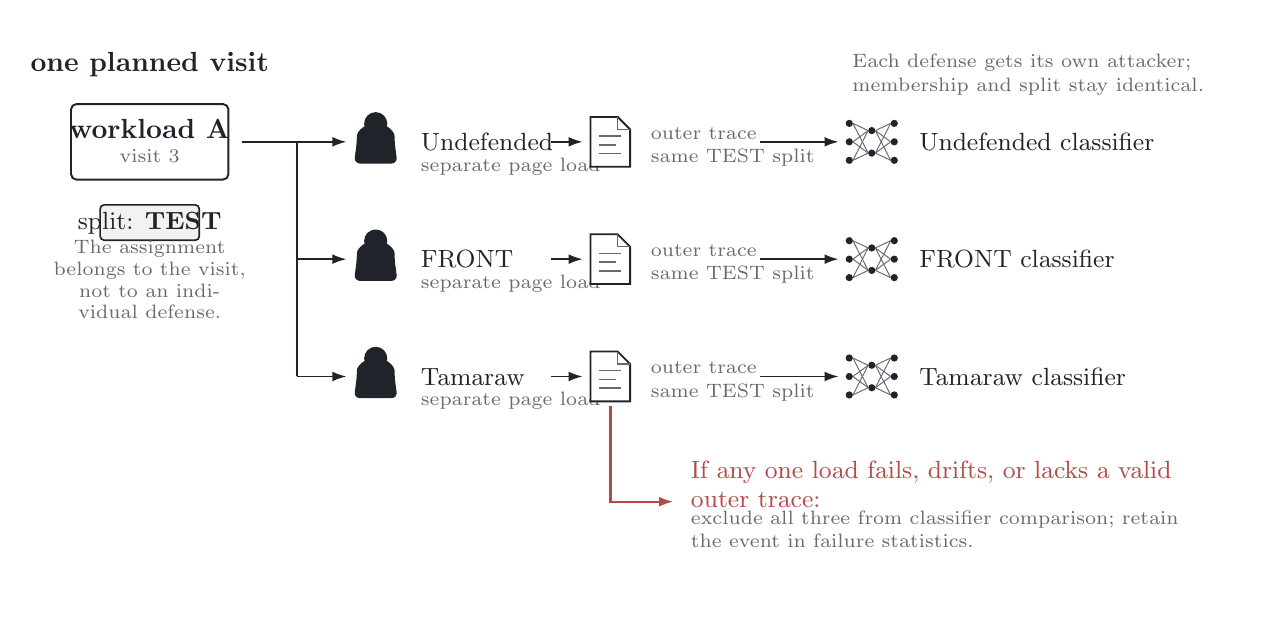
\begin{tikzpicture}[x=1cm,y=1cm]
  \QCSDSvgMetadata
    {Concrete paired visit and classifier split example}
    {Workload A visit 3 expands into undefended, FRONT, and Tamaraw page loads. All three share one test assignment and feed separately trained classifiers when their outer traces validate. Any failure or content drift excludes the entire paired visit from comparison but remains in failure statistics.}
  \path[use as bounding box] (0,0) rectangle (15.5,7.15);

  \node[caption,font=\bfseries] at (1.55,6.68) {one planned visit};
  \path[draw=qink,fill=white,line width=.7pt,rounded corners=2pt]
    (.55,5.22) rectangle (2.55,6.18);
  \node[caption,font=\bfseries] at (1.55,5.87) {workload A};
  \node[small note] at (1.55,5.52) {visit 3};
  \path[draw=qink,fill=qpale,line width=.6pt,rounded corners=1.5pt]
    (.92,4.45) rectangle (2.18,4.90);
  \node[caption] at (1.55,4.67) {split: \textbf{TEST}};
  \node[tiny note,align=center,text width=2.9cm] at (1.55,3.95)
    {The assignment belongs to the visit,\\not to an individual defense.};

  \draw[plain flow] (2.72,5.70) -- (3.42,5.70);
  \draw[plain flow] (3.42,2.72) -- (3.42,5.70);

  \foreach \y/\defense in {5.70/Undefended,4.21/FRONT,2.72/Tamaraw} {
    \draw[flow] (3.42,\y) -- (4.05,\y);
    \pic[scale=.92] at (4.42,\y) {client};
    \node[caption,anchor=west] at (4.87,\y) {\defense};
    \node[tiny note,anchor=west] at (4.87,{\y-.31}) {separate page load};

    \draw[flow] (6.65,\y) -- (7.05,\y);
    \pic[scale=.93] at (7.40,\y) {capture};
    \node[small note,anchor=west] at (7.79,{\y+.11}) {outer trace};
    \node[tiny note,anchor=west] at (7.79,{\y-.20}) {same TEST split};

    \draw[flow] (9.30,\y) -- (10.30,\y);
    \pic[scale=1.02] at (10.72,\y) {classifier};
    \node[caption,anchor=west] at (11.20,\y) {\defense\ classifier};
  }

  \node[small note,anchor=west,align=left] at (10.35,6.55)
    {Each defense gets its own attacker;\\membership and split stay identical.};

  \draw[failure] (7.40,2.35) -- (7.40,1.13) -- (8.20,1.13);
  \node[caption,text=qred,anchor=west,align=left,text width=6.4cm] at (8.30,1.35)
    {If any one load fails, drifts, or lacks a valid outer trace:};
  \node[small note,anchor=west,align=left,text width=6.4cm] at (8.30,.78)
    {exclude all three from classifier comparison; retain the event in failure statistics.};
\end{tikzpicture}
\end{document}
